\documentclass[main.tex]{subfiles}
\begin{document}
\chapter{Introduction}
\label{chapter:intro}

The Large Hadron Collider (LHC) at CERN has been colliding
particles since 2009, with each successive run increasing the centre-of-mass
energy of the collision, from 7 TeV in Run 1 to 13.6 TeV
at the time of writing. As the experiment has
operated for over a decade, there is a vast quantity of
experimental data collected that has to be compared with
theoretical predictions. Currently, the theory predictions
are made with the Standard Model (SM) of
particle physics which describes the fundamental particles
of nature and their interactions.

The standard paradigm for comparing
theory and experiment is to simulate the particle collisions
from the initial collision all the way through
to the detection of the hundreds of particles produced in the collision.
General purpose Monte Carlo event generators are the de facto
tool designed to generate these simulated events.
With the large number of scattering events collected at
the LHC already, and with even more expected at the High Luminosity LHC (HL-LHC),
the ability to generate the large simulated event samples
required for theory predictions within the available computing
budget presents a very real challenge.

The process of generating simulated events can be broadly
split up into three segments:
the highly energetic hard scattering process, 
the subsequent cascading of particles (parton shower),
and the formation of bound states detected (hadronisation),
which makes their way to the detectors.
While hadronisation is based on phenomenological models,
the hard scattering and parton shower are derived
from the SM and are perturbatively defined.

The hard scattering cross-section can be formulated as a probability
for particles to collide, represented by matrix elements.
These matrix elements are formally calculated order-by-order
in perturbation theory, with each order leading
to increasingly difficult computations at each order. In practice,
these matrix elements are provided in libraries interfaced
to the event generators and evaluation is largely automated for many
of the most important processes. However, the evaluation time
for these complex expressions becomes problematic
when generating the large samples required to compare with
experiments. Especially when a significant portion of the time
spent simulating an event is spent on evaluating matrix
elements.

The focus of this thesis will be on applying modern
machine learning methods to accelerate the evaluation
of matrix elements in order to speed up the event
generation process. Machine learning algorithms
have become ubiquitous in many fields, and their applicability
to a wide range of problems have made them a popular choice
in the high energy physics community as well. By combining the
well understood behaviour of matrix elements in specific
kinematic regions with powerful machine learning
algorithms, the construction of physics-inspired machine
learning models unlocks higher levels of accuracy
than would otherwise be achievable.

The structure of this thesis is as follows: in this chapter
I will recap the necessary concepts from the SM,
in particular quantum chromodynamics (QCD), the sector
which governs the behaviour of quarks and gluons. Furthermore,
I will elaborate on the relationship between theory and experiment
with the introduction of cross-sections, and their relation
to matrix elements.
In Chapter~\ref{chapter:qcd}, I will discuss the challenges that arise
in fixed-order perturbative calculations and the current methods
that have been adopted in the community to deal with them.
I will briefly introduce Monte Carlo event generators in
Chapter~\ref{chapter:MC}, where the theory discussed in the first
two chapters is applied in practice. In Chapter~\ref{chapter:ml},
I discuss how bottlenecks in traditional event generator techniques
motivates the usage of machine learning based approaches, with
particular attention placed on using neural networks as emulators
for matrix elements.
The construction of this neural network emulator is
described in detail in Chapter~\ref{chapter:fame1} for tree-level
electron-positron annihilation matrix element emulation.
A similar philosophy is applied in Chapter~\ref{chapter:fame2}
where next-to-leading order QCD k-factors are emulated for
the same processes.
These two chapters discuss in detail the procedure for
constructing emulators for electron-positron annihilation,
however, the more relevant processes for the LHC are in
proton-proton initiated collisions. The extension
to this scenario is detailed in Chapter~\ref{chapter:fame3}
where I also explore using the
emulator in a novel implementation to accelerate event unweighting
in the event generator {\Sherpa}.
Finally, I will summarise and conclude the thesis in
Chapter~\ref{chapter:conclusion}.

\section{The Standard Model of particle physics}
    The Standard Model of particle physics is our current
    best working theory to describe all known elementary particles,
    as well as three of the four fundamental forces. Developed
    predominantly in the latter half of the 20th century, it is
    one of the most well tested theories that we have in science today.
    Some highlights include the highly precise predictions of the
    anomalous magnetic moment of the electron, which agrees with experimental
    measurements to more than 10 significant figures \cite{Aoyama:2017uqe},
    and the discovery of the Higgs boson in 2012 by the ATLAS \cite{ATLAS:2012yve}
    and CMS experiments \cite{CMS:2012qbp} at the LHC,
    which was theorised decades prior.

    The SM is a gauge quantum field theory (QFT) where particles
    are described as excitations of quantum fields. The symmetry group
    of the SM is
    \begin{equation}\label{eqn:SM_gauge}
        \mathrm{SU}(3)_{c} \times \mathrm{SU}(2)_{L} \times \mathrm{U}(1)_{Y}\, ,
    \end{equation}
    where subscripts denote the charges of the gauge groups. The first gauge
    group with colour charge $c$ describes the interactions of the
    strong force within the theory of quantum chromodynamics, which we
    will elaborate more on in Section~\ref{sec:qcd}. The second
    and third gauge groups represent the electroweak sector of the SM, where
    $L$ denotes left-chiral fields that carry weak isospin, whilst $Y$ denotes
    the weak hypercharge. Under electroweak
    spontaneous symmetry breaking (EWSB), this product becomes
    \begin{equation}\label{eqn:SM_SSB}
        \mathrm{SU}(2)_{L} \times \mathrm{U}(1)_{Y} \xrightarrow{\mathrm{EWSB}} \mathrm{U}(1)_{\mathrm{EM}} \, ,
    \end{equation}
    giving rise to the electromagnetic and weak forces that we observe.
    The explanation of gravity in a QFT is an open problem and cannot currently
    be included in the SM as any Lagrangian including gravity cannot be renormalised.
    Fortunately, the effect of gravity is considered
    to be negligible on the scales considered at high energy colliders, and so it is ignored.
    Each of the three fundamental forces described by the SM is mediated
    by the exchange of a gauge boson. The massless gauge bosons mediating the strong
    and EM forces are the gluon $g$ and photon $\gamma$,
    respectively. For the weak force the gauge bosons are the $W^{\pm}$
    and $Z^{0}$ bosons, which attain a mass through the Higgs mechanism \cite{Englert:1964et,Higgs:1964pj,Guralnik:1964eu}
    during EWSB, elucidating the Higgs boson $H$.

    The matter content of the SM consists of fermions, which can be split
    into quarks and leptons. Quarks are massive and experience the strong,
    weak, and EM forces. Leptons are defined by their lack of colour charge,
    meaning they do not experience the strong force. Leptons can be separated
    into charged leptons (electron $e$, muon $\mu$, tau $\tau$
    and their antiparticles) which experience the weak and EM force, and 
    neutrinos (electron neutrino $\nu_{e}$, muon neutrino $\nu_{\mu}$, tau
    neutrino $\nu_{\tau}$ and their antiparticles) which only experience the
    weak force. Neutrinos are massless in the SM, however, they have been
    observed to have mass \cite{Super-Kamiokande:1998kpq,SNO:2002tuh}. This
    prompts physics beyond the Standard Model (BSM) to describe these observed masses.

    The particle content of the SM is summarised in Figure \ref{fig:SM_particles},
    which shows the quarks, leptons and bosons along with their masses, charges
    and spin.
    \begin{figure}
        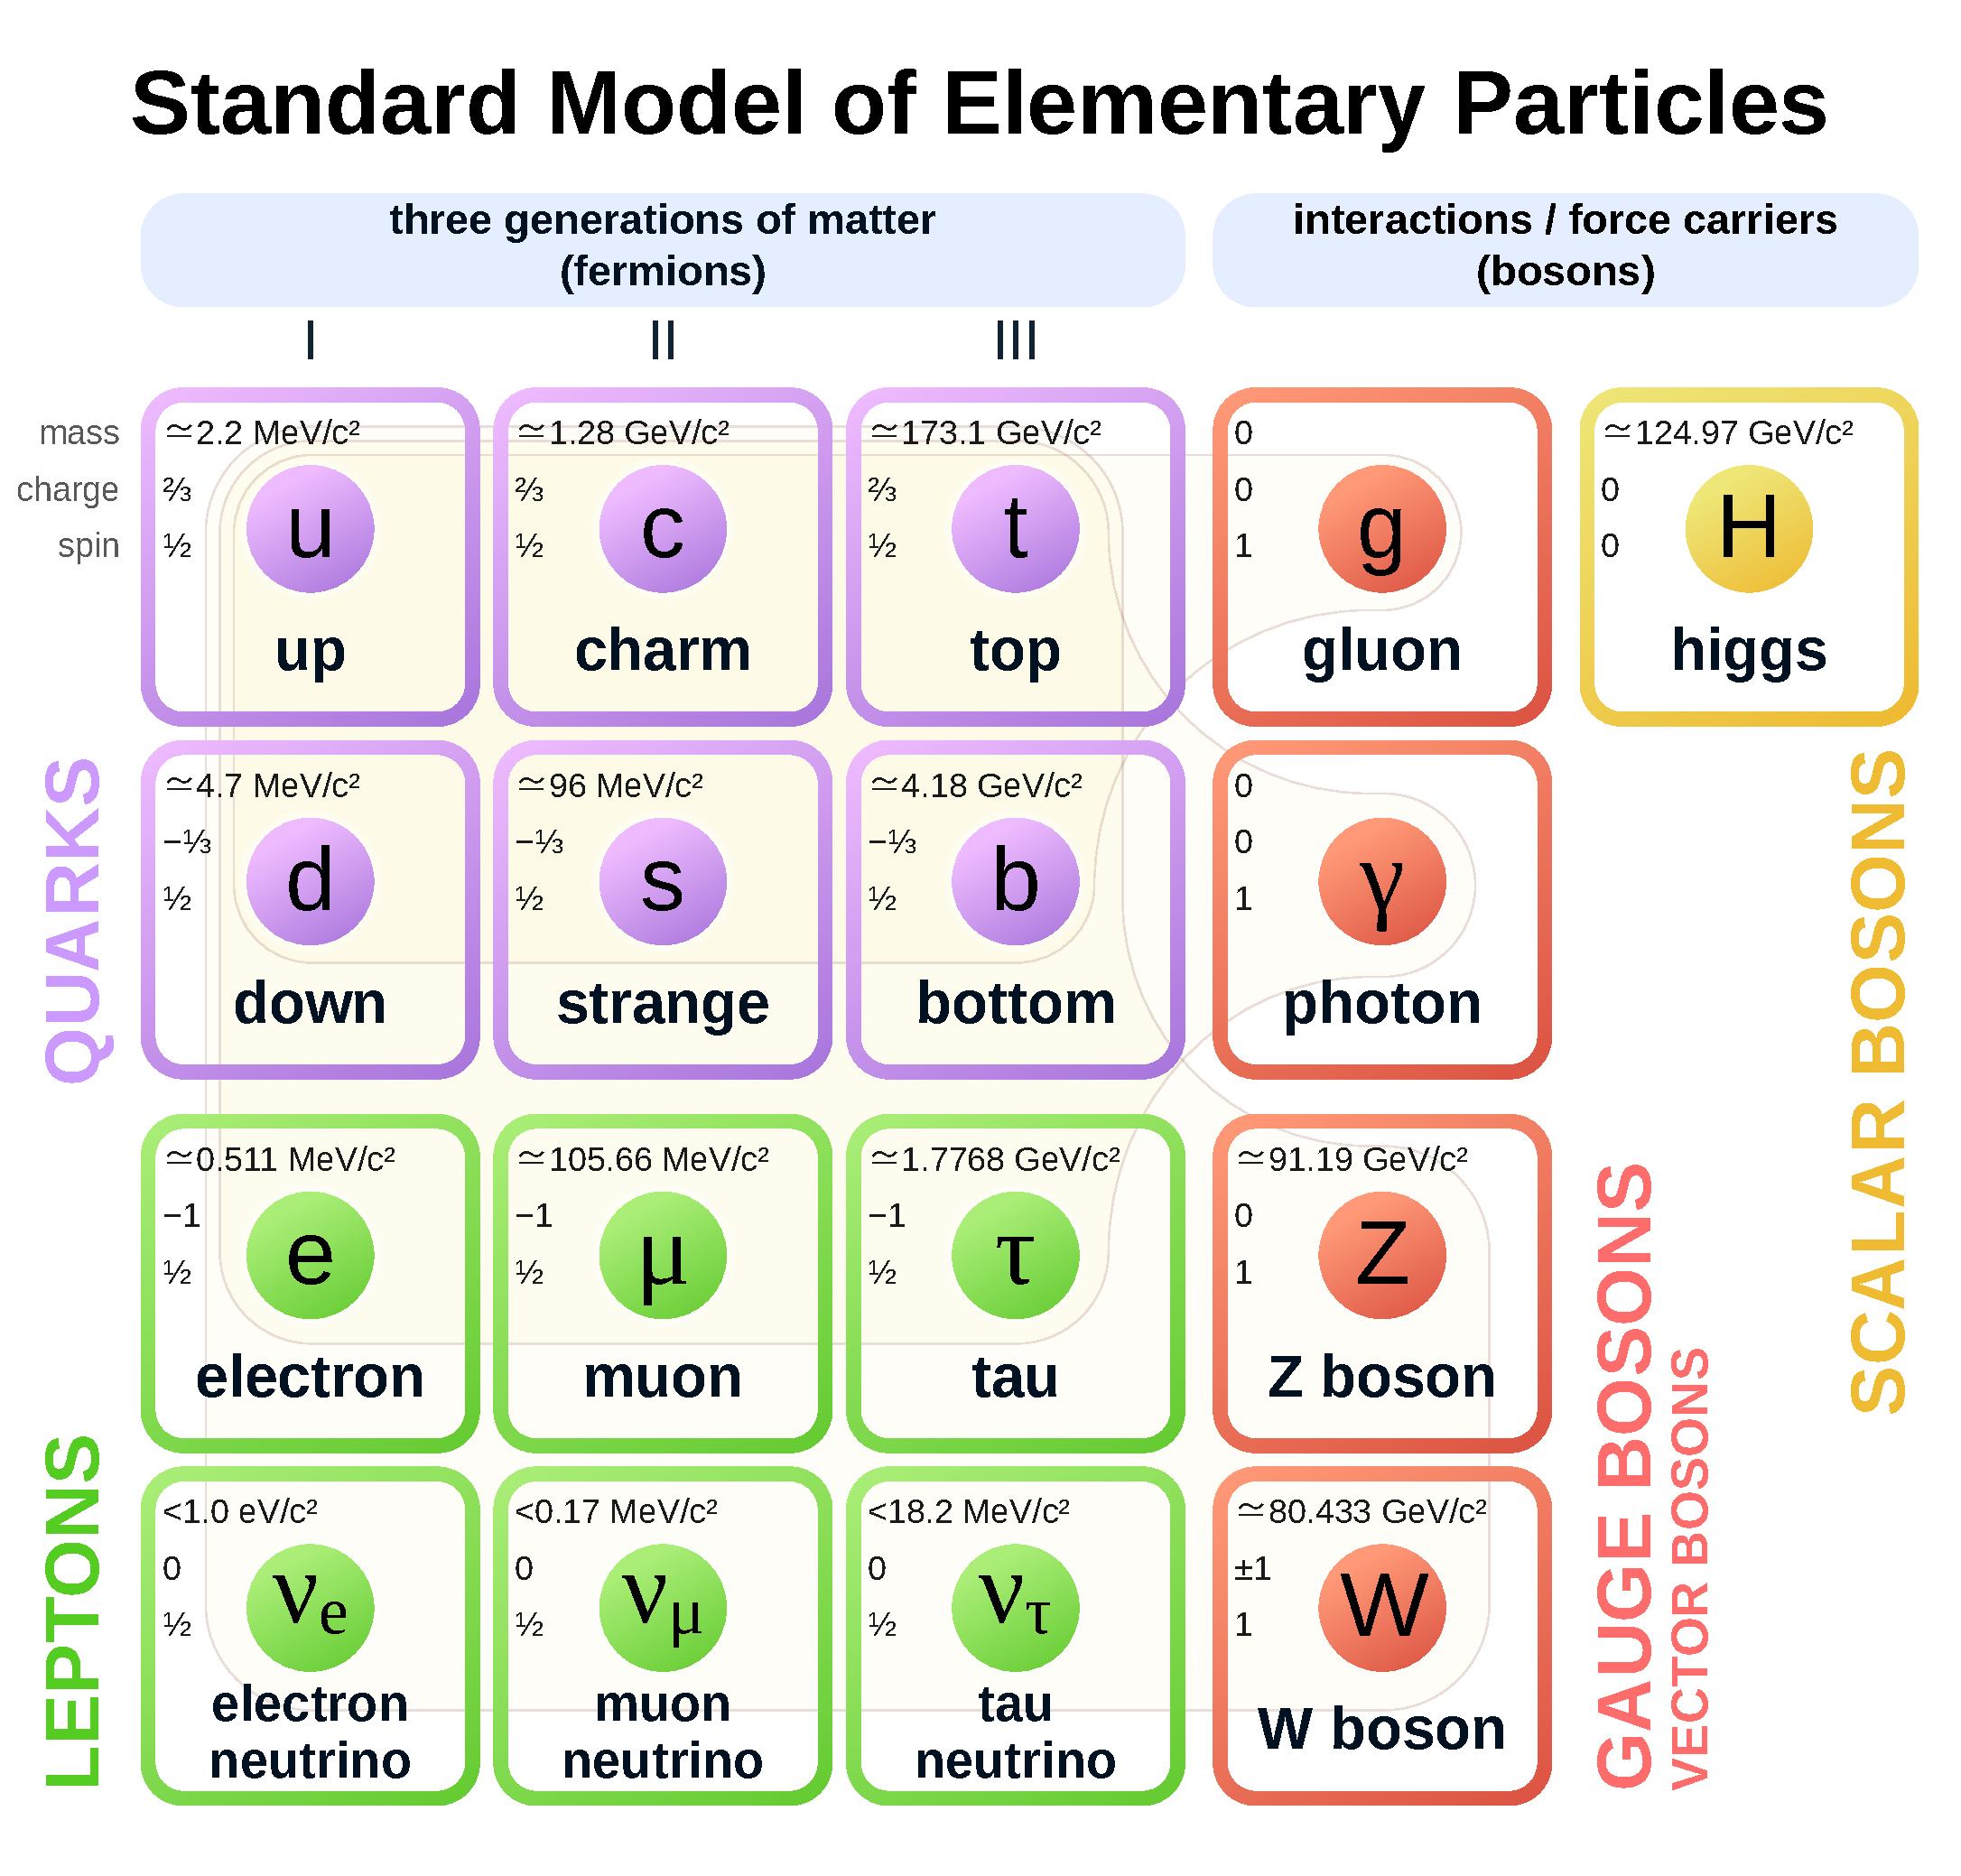
\includegraphics[width=\linewidth]{introduction/sm_particles.pdf}
        \caption{Particle content of the SM, split into quarks, leptons,
        gauge bosons and scalar bosons. The columns for the fermions depict
        the three different generations. The masses, electric charge, and spin
        are given for each particle. The yellow contours indicate the coupling
        of bosons to fermions, illustrating the forces experienced by the
        fermions inside the contour. Figure reproduced from \cite{SM_figure}.}
        \label{fig:SM_particles}
    \end{figure}
    The interactions of these fields are governed by the SM Lagrangian\footnote{Technically Lagrangian density but we use the terms
    Lagrangian and Lagrangian density interchangeably.}
    which can be written as
    \begin{equation}\label{eqn:L_SM}
        \mathcal{L}_{\mathrm{SM}} = \mathcal{L}_{\mathrm{gauge}} + \mathcal{L}_{\mathrm{fermion}} + \mathcal{L}_{\mathrm{Higgs}} + \mathcal{L}_{\mathrm{Yukawa}} + \mathcal{L}_{\mathrm{GF}} + \mathcal{L}_{\mathrm{ghost}} \, ,
    \end{equation}
    where $\mathcal{L}_{\mathrm{gauge}}$ describes the gauge fields,
    $\mathcal{L}_{\mathrm{fermion}}$ describes how fermions interact with
    gauge fields as well as their kinetic terms,
    $\mathcal{L}_{\mathrm{Higgs}}$ describes the Higgs field,
    $\mathcal{L}_{\mathrm{Yukawa}}$ describes the interactions between the Higgs
    field and fermions,
    $\mathcal{L}_{\mathrm{GF}}$ is a gauge fixing term,
    and $\mathcal{L}_{\mathrm{ghost}}$ is a ghost term.
    The last two terms are required to remove unphysical degrees of freedom
    when gauge fixing the theory.
    All terms in the SM Lagrangian are invariant under local transformations
    of the gauge group in Eq. (\ref{eqn:SM_gauge}).

    In the following section we will focus on the gauge, fermion, gauge-fixing
    and ghost Lagrangian terms in the framework of QCD, which is the most
    relevant sector for this thesis. The remaining terms are discussed at
    length in standard reference texts \cite{Peskin:1995ev,Schwartz:2014sze,Romao:2012pq}.


\section{Introduction to quantum chromodynamics}\label{sec:qcd}
    \subsection{The QCD Lagrangian}\label{sec:L_qcd}
    Quantum chromodynamics is the sector of the SM that
    describes the strong interaction. 
    QCD is a non-Abelian gauge theory with gauge group
    $\mathrm{SU}(N_{c} = 3)$ where the charge is named colour.
    The gauge and fermion part of the QCD Lagrangian is
    \begin{equation}\label{eqn:L_QCD}
        \mathcal{L}_{\mathrm{QCD}} = -\dfrac{1}{4}F^{a}_{\mu\nu}F^{a, \, \mu\nu}
        + \sum_{f} \bar{\psi}_{i}^{f}(\mathrm{i}\slashed{D}_{ij} - \delta_{ij}m_{f})\psi_{j}^{f} \, ,
    \end{equation}
    where repeated indices are summed over.
    The fields $\psi_{i}^{f}$ are the fermions field operators,
    representing quarks and antiquarks with flavours $f$: 
    up $u$, down $d$, strange $s$, charm $c$, top $t$, and bottom $b$,
    with masses $m_{f}$. The field operators transform under the fundamental
    representation with indices $i, j \in \{1, 2, 3\}$, named colour indices.
    The gauge fields $A^{a}_{\mu}$, corresponding to gluons, 
    appear in the quark covariant derivative
    \begin{equation}\label{eqn:covariant_deriv}
        (D_{\mu})_{ij} = \delta_{ij}\partial_{\mu} - \mathrm{i}g_{s}T^{a}_{ij}A^{a}_{\mu} \, ,
    \end{equation}
    and the gauge field strength tensor
    \begin{equation}\label{eqn:F_munu}
        F^{a}_{\mu\nu} = \partial_{\mu}A^{a}_{\nu} - \partial_{\nu}A^{a}_{\mu} + g_{s} f^{abc}A^{b}_{\mu}A^{c}_{\nu} \, .
    \end{equation}
    Gauge fields transform under the adjoint representation, 
    which is an $N_{c}^{2}-1$ dimensional representation such that
    the adjoint indices $a,b,c \in \{1,...,8\}$. $T^{a}_{ij}$ are the
    group generators in the fundamental representation. In SU(3) it is
    common to write the group generators as
    \begin{equation}\label{eqn:group_generators}
        T^{a}_{ij} = \dfrac{1}{2}\lambda^{a}_{ij}
    \end{equation}
    where $\lambda^{a}_{ij}$ are the Gell-Mann matrices \cite{Gell-Mann:1962yej}.
    The generators of the group obey the Lie algebra
    \begin{equation}\label{eqn:lie_algebra}
        [T^{a}, T^{b}] = \mathrm{i}f^{abc}T^{c} \, ,
    \end{equation}
    where $f^{abc}$ are the structure constants of SU(3).
    By convention, the generators are normalised to be
    \begin{equation}\label{eqn:generator_normalisation}
        \mathrm{Tr}(T^{a}T^{b}) = \delta^{ab}T_{R} \, , \quad \mathrm{where} \quad T_{R} = \dfrac{1}{2} \, .
    \end{equation}
    This normalisation sets the values of the Casimirs
    of the group as
    \begin{align}\label{eqn:casimirs}
        \begin{split}
            T^{a}_{ij}T^{a}_{jk} &= \delta_{ik}C_{F} \, , \quad C_{F} = \dfrac{N_{c}^2-1}{2N_{c}} \, , \\
            f^{abc}f^{abd} &= \delta^{cd}C_{A} \, , \quad C_{A} = N_{c} \, ,
        \end{split}
    \end{align}
    where $C_{F}=4/3$ and $C_{A}=3$ for QCD.
    These are collectively referred to as colour factors.

    The gauge coupling of the group $g_{s}$
    is a dimensionless free parameter of the theory.
    It is common to use the strong coupling constant
    instead, 
    \begin{equation}\label{eqn:alpha_s}
        \alpha_{s} = \dfrac{g_{s}^{2}}{4\pi} \, .
    \end{equation}
    The strong coupling constant is in fact not constant, and
    depends on the energy scale of the process. This
    is due to the process of renormalisation, which will be discussed
    in Section~\ref{sec:renormalisation}.
    The implication of this is that at collider
    experiments where collisions occur at extremely high energy,
    the strong coupling constant becomes small, a
    property known as asymptotic freedom. A consequence
    of this is that predictions made in QCD can be expressed
    in the form of perturbative expansions in $\alpha_{s}$ (see Section~\ref{sec:xs}).

    To remove unphysical degrees of freedom from the
    theory we need to fix the gauge
    and add a ghost Lagrangian. The gauge-fixing term
    in the $R_{\xi}$ gauge is written as
    \begin{equation}\label{eqn:L_GF}
        \mathcal{L}_{\mathrm{GF}} = -\dfrac{1}{2\xi}(\partial^{\mu}A_{\mu}^{a})^{2} \, ,
    \end{equation}
    where $\xi = 1$ corresponds to the Feynman-'t Hooft gauge.
    Ghosts and antighosts are anti-commuting fields
    introduced for each gauge field as a way to conveniently compute
    determinants occurring in the gauge fixing procedure.
    The ghost Lagrangian is most commonly written
    in the Faddeev-Popov procedure as
    \begin{equation}\label{eqn:L_ghost}
        \mathcal{L}_{\mathrm{ghost}} = (\partial_{\mu}\bar{c}^{a})(\delta^{ac}\partial_{\mu} + g_{s}f^{abc}A^{b}_{\mu})c^{c} \, ,
    \end{equation}
    where $c^{a}$ ($\bar{c}^{a}$) are Faddeev-Popov ghosts (antighosts).
    Ghosts are particles that subtract the longitudinal
    degree of freedom from gluons, and as such it is usual to
    use them to cancel the longitudinal degree of freedom of gluon propagators.
    It should be noted that ghosts could in principle be included as external states as well
    for the same purpose, however, it is more conventional to use the usual physical polarisation sum
    instead.

    \subsection{QCD Feynman rules}\label{sec:qcd_feynman}
    Now that we have written down the QCD Lagrangian,
    we can examine the terms that govern the interactions between
    bosons and fermions, and especially
    important for QCD, the gauge boson self interactions. A convenient
    way to do this is by deriving the Feynman rules of the theory, which can be
    pieced together to form Feynman diagrams. We will see
    that Feynman diagrams are a simple but powerful tool
    to systematically build up all the possible ways in which a process
    can occur.

    Expanding Eq. (\ref{eqn:L_QCD}) and extracting the terms
    that mix the gauge and fermion fields, we get an interaction Lagrangian
    \begin{equation}\label{L_int}
        \mathcal{L}_{\mathrm{int}} = g_{s}A^{a}_{\mu}\bar{\psi}_{i}^{f}\gamma^{\mu}T^{a}_{ij}\psi_{j}^{f}-g_{s}f^{abc}(\partial_{\mu}A^{a}_{\nu})A^{b,\,\mu}A^{c,\,\nu} -\dfrac{g_{s}^{2}}{4}f^{abc}A^{b}_{\mu}A^{c}_{\nu}f^{ade}A^{d,\,\mu}A^{e,\,\nu} \, ,
    \end{equation}
    which we can interpret as follows: the first term
    is an interaction between a gluon and two fermion field operators,
    the second term is a three gluon
    self-interaction, and the third term is a four gluon
    self-interaction. These mixing terms can be recast
    into Feynman rules representing interaction vertices.

    To connect vertices we require propagators, which
    we can read off from the kinetic Lagrangian where
    we collect terms from Eqs. (\ref{eqn:L_QCD}) and (\ref{eqn:L_GF}), 
    \begin{equation}\label{L_kin}
        \mathcal{L}_{\mathrm{kin}} = -\dfrac{1}{4}(\partial_{\mu}A^{a}_{\nu}-\partial_{\nu}A^{a}_{\mu})^{2} - \dfrac{1}{2\xi}(\partial_{\mu}A^{a}_{\mu})^{2} + \bar{\psi}_{i}^{f}(\mathrm{i}\slashed{\partial}-m_{f})\psi_{i}^{f} \, ,
    \end{equation}
    where the first two terms corresponds to a gluon
    propagator and the third term corresponds to
    a quark propagator.

    \begin{figure}
        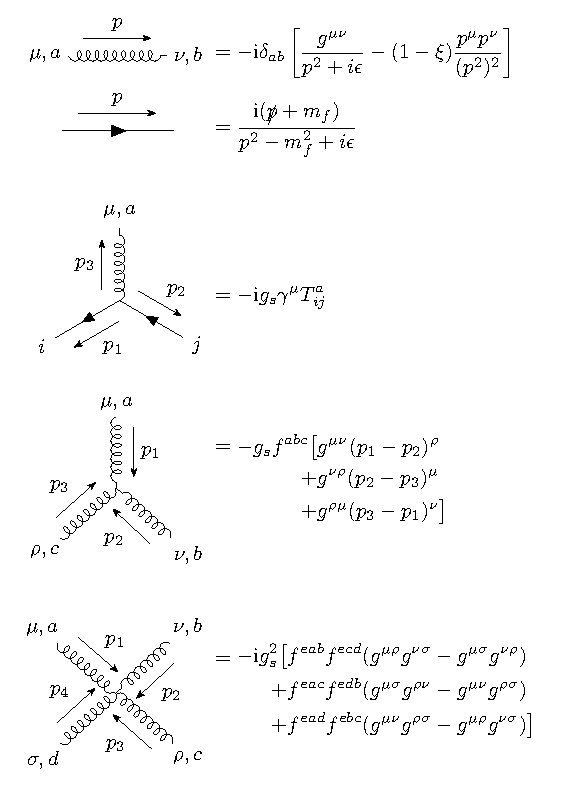
\includegraphics[width=\linewidth]{introduction/qcd_feynman_rules.pdf}
        \caption{QCD Feynman rules with the Minkowski metric $g^{\mu\nu} = \mathrm{diag}(1, -1, -1, -1)$.}
        \label{fig:qcd_feynman_rules}
    \end{figure}

    From these Lagrangians, we can read off the QCD Feynman rules
    which we have collected in Figure~\ref{fig:qcd_feynman_rules}.
    Note that we have only written down the vertices and propagators
    for the physical gluons and quarks.
    Ghosts also have associated Feynman rules but we do
    not specify those here. A full list of Feynman rules
    in the SM can be found in Ref. \cite{Romao:2012pq}.

    From these Feynman rules, we identify that each
    fermion-gluon and three gluon vertex
    is associated with one power of $\alpha_{s}$ (due to squaring $g_{s}$),
    and the four gluon vertex is associated with
    two powers of $\alpha_{s}$. This relationship
    between vertices and $\alpha_{s}$ allows
    us to systematically build up Feynman diagrams
    that correspond to a fixed-order in $\alpha_{s}$.
    This point will be elaborated on in Section
    \ref{sec:xs} where we discuss scattering amplitudes
    and how they are related to Feynman diagrams.

\section{Factorisation theorem}\label{sec:factorisation}
    At the LHC collisions occur between two protons,
    which have constituent quarks and gluons, collectively
    named partons.
    The application of QCD to describe phenomena
    in these proton-proton collisions rests on the use of
    the factorisation theorem, which enables the
    separation of low and high energy scales (so-called soft and hard).
    Within the proton, there are quarks-antiquark pairs
    and gluons that are constantly absorbed and
    emitted on a timescale inversely proportional
    to the mass of the proton.
    The timescale of this fluctuation is much longer
    than the timescale of the interaction between
    a parton and a highly energetic probing parton
    from another proton. This is the scenario
    that occurs in collisions at the LHC.
    During the collision, or the hard scattering,
    the probe is able to interact with a
    parton that is effectively frozen.
    The probing parton knows nothing of the
    proton being probed, except for the fact
    that it collided with a parton carrying
    a fraction of the proton momentum. The
    distribution of partons within a proton
    is process independent and a fundamental
    property of the proton, meaning it can be
    separated from the actual scattering between
    the partons.

    This heuristic argument motivates the form of
    the factorisation equation, where the cross-section,
    which is proportional to the production rate of
    particles from a hadronic collision, can be written as
    \begin{equation}\label{eqn:hadronic_cs}
        \sigma_{AB \rightarrow n} = \sum_{a, b}\int_{0}^{1} \mathrm{d}x_{a}\mathrm{d}x_{b} \; f_{a/A}(x_{a},\mu_{F})f_{b/B}(x_{b}, \mu_{F}) \; \hat{\sigma}_{ab \rightarrow n}(Q, \mu_{F}, \mu_{R}) + \mathcal{O}\left(\dfrac{\Lambda_{\mathrm{QCD}}}{Q}\right)\, ,
    \end{equation}
    where $a$ is the parton from hadron $A$,
    and $b$ is the parton from hadron $B$.
    The sum over initial-state partons $a$ and $b$
    indicates the sum over flavours, which depends
    on the hadron composition in general.
    This factorisation is not exact as indicated by the
    correction term, which is inversely proportional to the characteristic
    hard scale $Q$. The other scale involved, $\Lambda_{\mathrm{QCD}}$, the QCD scale,
    is the scale at which $\alpha_{s}$ becomes
    large enough that perturbation theory breaks down.
    However, for high energy collisions, where
    $Q \gg \Lambda_{\mathrm{QCD}}$, this term and higher order
    terms are suppressed.
    In fact, the factorisation equation has only been
    proven for a few specific cases \cite{Collins:2011zzd,Collins:1987pm,Collins:1989gx,Amoroso:2022eow}.

    The parton distribution functions (PDFs), $f_{a/h}(x, \mu)$,
    depend on the momenta fraction $x$ carried by parton $a$,
    with respect to its parent hadron $h$, at a scale $\mu$,
    usually taken to be the factorisation scale $\mu_{F}$.
    The factorisation scale is the interface between soft and hard physics.
    The interpretation of PDFs at leading order are
    as probability distributions: $f_{a/h}(x, \mu)$ is
    the probability of finding parton $a$ within $h$
    carrying a momentum fraction $x$ at the energy scale $\mu$.
    PDFs are non-perturbative objects that encapsulate
    the soft effects of the scattering occurring below energy
    $\mu_{F}$. They are non-perturbative because
    they are determined by fitting to experimental data,
    instead of being calculated in perturbation theory.
    
    For a review of PDFs and how they are determined
    see Refs. \cite{Ethier:2020way,Jimenez-Delgado:2013sma}.
    In practice, these PDF fits are accessed through the
    LHAPDF interface \cite{Buckley:2014ana} which provides
    PDF sets from multiple working groups \cite{PDF4LHCWorkingGroup:2022cjn,Hou:2019efy,Bailey:2020ooq,NNPDF:2021njg}.
    The evolution of PDFs between factorisation scales is possible
    through the use of the Dokshitzer-Gribov-Lipatov-Altarelli-Parisi (DGLAP)
    equations \cite{Dokshitzer:1977sg,Gribov:1972ri,Lipatov:1974qm,Altarelli:1977zs},
    \begin{equation}\label{eqn:DGLAP}
        \mu_{F}^{2} \dfrac{\partial}{\partial \mu_{F}^{2}}
        \begin{pmatrix}
            f_{q/h}(x,\mu_{F}) \\
            f_{g/h}(x,\mu_{F})
        \end{pmatrix} \\
        = \dfrac{\alpha_{s}(\mu_{F})}{2\pi} \int_{x}^{1} \dfrac{\mathrm{d}z}{z}
        \begin{pmatrix}
            P_{qq}(\frac{x}{z}) & P_{qg}(\frac{x}{z}) \\
            P_{gq}(\frac{x}{z}) & P_{gg}(\frac{x}{z})
        \end{pmatrix}
        \begin{pmatrix}
            f_{q/h}(z,\mu_{F}) \\
            f_{g/h}(z,\mu_{F})
        \end{pmatrix} \, ,
    \end{equation}
    where $P_{ab}(\frac{x}{z})$ are splitting functions
    representing parton $b$ emitting a parton $a$, that carries
    a momentum fraction $x$. These splitting functions are calculable
    as a power series in $\alpha_{s}$ where they have been computed
    up to three-loops \cite{Moch:2004pa,Vogt:2004mw}.
    At leading order they are \cite{Altarelli:1977zs}
    \begin{equation}\label{eqn:AP_kernels}
        \begin{split}
            P^{(0)}_{qq}(z) &= C_{F}\left[\dfrac{1+z^{2}}{(1-z)_{+}} + \dfrac{3}{2}\delta(1-z)\right] \, , \\
            P^{(0)}_{qg}(z) &= T_{R}\left[z^{2} + (1-z)^{2}\right] \, ,\\
            P^{(0)}_{gq}(z) &= C_{F}\left[\dfrac{1+(1-z)^{2}}{z^{2}}\right] \, ,\\
            P^{(0)}_{gg}(z) &= 2C_{A}\left[\dfrac{z}{(1-z)_{+}}+\dfrac{1-z}{z}+z(1-z)\right] + \left(\dfrac{11C_{A}-4T_{R}n_{f}}{6}\right)\delta(1-z) \, ,
        \end{split}
    \end{equation}
    where the divergences at $z=1$ have been regulated
    with the `$+$'-prescription, which is defined as
    \begin{equation}\label{eqn:plus_prescription}
        \int_{0}^{1} \mathrm{d}z \; [g(z)]_{+}f(z) = \int_{0}^{1}\mathrm{d}z \; g(z)(f(z)-f(1)) \, .
    \end{equation}
    With this prescription, the divergence at $g(z=1)$ is cancelled,
    given that the function $f(z)$ is sufficiently smooth at $z=1$.
    At leading order, there is a physical interpretation
    of the splitting kernels as the probability of finding a parton
    $a$ in parton $b$ carrying a momentum fraction $x$ of the parent parton.
    
    The momentum fractions, $x$, also link the
    squared centre-of-mass energies of the hadronic collision,
    denoted as $s$, to the partonic equivalent as
    \begin{equation}\label{eqn:E_cm_partonic}
        \hat{s} = x_{a}x_{b}s \, .
    \end{equation}
    The partonic cross-section, $\hat{\sigma}_{ab \rightarrow n}(Q, \mu_{F}, \mu_{R})$,
    describes the interaction of
    partons $a$ and $b$ scattering into $n$ particles,
    where the scattering occurs at energy scale $Q$,
    which is often taken to be $\hat{s}$.
    Notice that the partonic cross-section depends on
    both the factorisation scale, $\mu_{F}$, and
    the renormalisation scale, $\mu_{R}$
    (see Section~\ref{sec:renormalisation}). This dependence will
    be discussed in Section~\ref{sec:scale_variations}
    in the context of theoretical uncertainties.

    The discussion so far has been focused on hadron-hadron
    initiated scattering, however a similar argument
    can be made about electron-positron annihilation,
    where the electron-positron annihilates to form a
    photon or $Z$ boson which decays into a quark-antiquark
    pair. For a sufficiently high energy collision,
    these interactions can be calculated in perturbation
    theory.
    Although electrons and positrons are fundamental
    particles and not composite particles, the 
    cross-sections in electron-positron collisions
    have contributions from the initial-state radiation,
    which also reduces the energy of the hard scattering.
    One method to capture these effects is through
    the use of process-independent structure functions \cite{Kuraev:1985hb}
    which are analogous to PDFs. Therefore, the discussion
    presented in this section applies to electron-positron
    cross-sections as well.
    
    We have seen that cross-section computations involve
    the convolution of PDFs with partonic cross-sections,
    $\hat{\sigma}_{ab \rightarrow n}$, which are
    calculated in perturbation theory.
    The details of how partonic cross-sections
    are computed is discussed in the next section.

\section{Scattering amplitudes and cross-sections}\label{sec:xs}
    At collider experiments we typically collide
    two beams consisting of bunches of energetic
    particles and analyse the resulting products
    of these collisions. The predictions that we make
    from our theoretical model are the partonic
    cross-sections. To arrive at an expression
    for the partonic cross-section, we need to
    first consider the hard scattering of particles.
    To model the hard collisions in
    a collider experiment, we look at the specific
    case of two particles colliding and producing $n$ particles.
    Scattering amplitudes are used to mathematically
    describe these scattering processes.
    For an initial-state
    $|i\rangle$ and final-state $|f\rangle$
    the scattering amplitude can be written as
    the overlap between the states
    \begin{equation}\label{eqn:scattering}
        \langle f | S | i \rangle \, ,
    \end{equation}
    where the scattering matrix, or $S$-matrix
    can be decomposed into an identity matrix
    and a transfer matrix $\mathcal{T}$,
    \begin{equation}\label{eqn:S_matrix}
        S = \mathbbm{1} + \mathrm{i}\mathcal{T} \, .
    \end{equation}
    The $S$-matrix encodes all the information
    about how the initial-state will evolve
    over time. By writing
    the $S$-matrix in this way, all the interactions
    are separated into the transfer matrix $\mathcal{T}$,
    as the identity matrix describes the free theory.
    By imposing a momentum conservation constraint
    on the $S$-matrix, the matrix element,
    $\mathcal{M}$, is defined in the following expression
    \begin{equation}\label{eqn:S_matrix_element}
        \langle f | \mathcal{T} | i \rangle = (2\pi)^{4} \delta^{4}\left(p_{a} + p_{b} - \sum_{f=1}^{n} p_{f}\right) \mathcal{M} \, ,
    \end{equation}
    where we take $p_{a}$ and $p_{b}$ to be
    the momenta of the two colliding
    particles in the initial-state, and $p_{f}$ to be the
    momenta of the $n$ particles in the final-state.
    The probability of this process occurring
    is the modulus squared of the scattering amplitude\footnote{Neglecting the case of scattering with no interactions taking place.}
    \begin{equation}\label{eqn:S_prob}
        P = |\langle f | S | i \rangle|^{2} \propto | \langle f | \mathcal{M} | i \rangle |^{2}
    \end{equation}
    where $|\langle f | \mathcal{M} | i \rangle|^{2}  \equiv |\mathcal{M}|^{2}$
    is the matrix element squared\footnote{Henceforth we refer to the matrix
    element squared as matrix element, unless stated otherwise.}.
    
    An observable that can be measured at experiments is
    the cross-section, $\sigma$, as introduced in
    Eq. (\ref{eqn:hadronic_cs}). The cross-section is a property
    of the particles being scattered, and is independent
    of the way the experiment is carried out (disregarding energy scale of experiment).
    Since the hadronic cross-section factorises
    the low energy effects into the non-perturbative PDFs,
    which are determined once, for all
    processes, the object of interest now becomes the
    partonic cross-section, $\hat{\sigma}$, which
    encodes the scattering information of the specific
    process considered.

    Given that cross-sections are measurable
    quantities, the partonic cross-section directly
    relates the matrix elements which we calculate in our QFT
    to measurable observables at experiments.
    In practice, it is more useful to consider the
    differential cross-section, $\mathrm{d}\hat{\sigma}$,
    where the cross-section can be differential
    in quantities such as energies and angles.
    This is because individual events at experiments
    will be measured to be in a specific interval of
    the differential quantity, meaning differential
    cross-sections can be plotted as histograms. Predictions
    can then be made on the theory side by binning simulated
    events.

    The differential partonic cross-section can be written as
    \begin{equation}\label{eqn:dsigma}
        \mathrm{d}\hat{\sigma} = \dfrac{1}{\mathcal{F}}|\mathcal{M}_{ab \rightarrow n}|^{2} \mathrm{d}\Phi_{n} \, ,
    \end{equation}
    where the flux factor, $\mathcal{F}$, is given by
    \begin{equation}\label{eqn:flux}
        \mathcal{F} = 4\sqrt{(p_{a}p_{b})^{2} - m_{a}^{2}m_{b}^{2}} \, .
    \end{equation}
    In the massless limit the flux factor reduces reduces to
    \begin{equation}\label{eqn:massless_flux}
        \mathcal{F} = 2(p_{a} + p_{b})^{2} = 2\hat{s} \, .
    \end{equation}
    It is common to use the massless limit because
    the centre-of-mass energy of a collider
    experiment is much greater than the mass
    of the colliding particles, and so we can
    neglect the masses.

    The Lorentz-invariant phase-space, $\mathrm{d}\Phi_{n}$,
    contains all the possible
    configurations of the $n$-particle final-state.
    Absorbing the momentum conserving $\delta$-function
    from Eq. (\ref{eqn:S_matrix_element}),
    we can write it as
    % \begin{equation}\label{eqn:dlips}
    %     \mathrm{d}\Phi_{n} = (2\pi)^{d}\delta^{(d)}\left(p_{a} + p_{b} - \sum_{f} p_{f}^{\mu}\right) \prod_{f=1}^{n} \dfrac{\mathrm{d}^{d}p_{f}}{(2\pi)^{d-1}}\delta(p_{f}^{2} - m_{f}^{2})\theta(E_{f}) \, ,
    % \end{equation}
    \begin{equation}\label{eqn:dlips_4d}
        \mathrm{d}\Phi_{n} = (2\pi)^{4}\delta^{4}\left(p_{a} + p_{b} - \sum_{f=1}^{n} p_{f}\right) \prod_{f=1}^{n} \dfrac{\mathrm{d}^{4}p_{f}}{(2\pi)^{3}}\delta(p_{f}^{2} - m_{f}^{2})\theta(E_{f}) \, ,
    \end{equation}
    where the second $\delta$-function restricts
    the final-state particles to be on mass-shell
    (on-shell), and the step function selects only
    the positive energy solution.
    This gives an intuitive picture of the partonic
    cross-section as the probability of a $2\rightarrow n$
    process occurring, summed over all the possible
    valid final-state configurations.

    From the definition of the transition probability
    Eq. (\ref{eqn:S_prob}), it becomes clear
    that the matrix element is the object which
    relates back to the Lagrangian of the theory
    as it encodes the interactions of the particles.
    We saw in Section \ref{sec:qcd_feynman} that
    interactions could be codified into Feynman
    rules which are pieced together to construct
    Feynman diagrams. In this picture, matrix elements
    are exactly the sum over all Feynman diagrams\footnote{Since we are working on the level
    of $|\mathcal{M}|^{2}$, this would
    be the sum of all interference terms.}
    for a particular process. However, for a given
    process the exact matrix element is a sum over
    infinitely many Feynman diagrams.
    Fortunately, because $\alpha_{s}$
    is small in high energy collisions, we can expand
    the matrix element as a perturbative series in
    $\alpha_{s}$ to write
    \begin{equation}\label{eqn:matrix_element}
        |\mathcal{M}|^{2} =  \alpha_{s}^{m} |\mathcal{M}|^{2}_{\mathrm{LO}} + \alpha_{s}^{m+1} |\mathcal{M}|^{2}_{\mathrm{NLO}} + \alpha_{s}^{m+2} |\mathcal{M}|^{2}_{\mathrm{NNLO}} + \mathcal{O}(\alpha_{s}^{m+3}) \, ,
    \end{equation}
    where $m$ corresponds to the powers of $\alpha_{s}$
    in the simplest Feynman diagrams
    for the process of interest.
    Since each term of this expansion is at a fixed-order
    in $\alpha_{s}$, it is possible to systematically
    compute the diagrams which contribute at the given order of $\alpha_{s}$.
    The set of diagrams that contribute at the lowest
    order in $\alpha_{s}$ are $|\mathcal{M}|^{2}_{\mathrm{LO}}$,
    where LO stands for leading order. The next term
    in the expansion corresponds to the leading order
    diagrams with an additional loop, or external leg,
    which contributes an extra factor of $\alpha_{s}$.
    This term is dubbed NLO for next-to-leading order
    in $\alpha_{s}$, and the following term
    next-to-next-to-leading order has again an additional
    loop or leg. In general, we have terms
    N$^{k}$LO where each additional power of $\alpha_{s}$
    increases complexity of the computations, however,
    because $\alpha_{s}$ is small, each additional term
    should contribute less and less.
    In principle, this means that the first terms dominate the expansion,
    and it should be sufficient to terminate the series after
    a few terms to reach an acceptable level of accuracy.

    In summary, the partonic cross-section of a collision
    reduces to the computation of the matrix elements
    up to a fixed-order in the coupling parameter,
    which is then integrated over the valid phase-space of
    final-state particle configurations. For hadronic
    collisions the partonic cross-section also needs to
    be convolved with the PDFs to obtain the hadronic
    cross-sections.

    With the introduction of matrix elements and
    cross-sections complete, we will move the discussion onto
    more practical aspects of computations within the
    QCD framework. More specifically, we will discuss
    the divergent structure of matrix elements
    and the machinery developed to tackle these
    unphysical singularities.

\end{document}